
% this file is called up by thesis.tex
% content in this file will be fed into the main document

%: ----------------------- introduction file header -----------------------
\begin{savequote}[50mm]
Historical methodology, as I see it, is a product of common sense applied to circumstances. 
\qauthor{Samuel E. Morison}
\end{savequote}


\chapter{Método para la evaluación de competencias genéricas}
\label{cha:Overall methodology}

% the code below specifies where the figures are stored
\ifpdf
    \graphicspath{{4_overall_methodology/figures/PNG/}{4_overall_methodology/figures/PDF/}{4_overall_methodology/figures/}}
\else
    \graphicspath{{4_overall_methodology/figures/EPS/}{4_overall_methodology/figures/}}
\fi

%------------------------------------------------------------------------- 

En este capítulo se propone un método para la evaluación de competencias genéricas de los estudiantes basado en el diseño de evaluaciones a partir de la actividad de estos en los entornos de aprendizaje. Se describe el método, sus características, los requisitos que el método ha de satisfacer y se introduce el tipo de herramienta que se empleará para su implementación.

\section{Introducción}

Se podría decir que hoy en día los entornos virtuales constituyen una pieza fundamental en cualquier contexto en el que se impartan cursos. Mientras que en los cursos virtuales, los VLEs son el único entorno de trabajo posible, en los cursos presenciales o mixtos, tantos los VLEs como otras herramientas virtuales actúan como soporte virtual de las clases, proporcionando multitud de actividades de aprendizaje. 

En esta tesis se propone un método de evaluación de competencias genéricas basado en el diseño de evaluaciones (DBA, del inglés, \emph{design-based assessment}) y que tiene su origen en la investigación basada en el diseño (DBR). DBA es un método de evaluación de competencias genéricas que se basa en indicadores de la actividad generada por los estudiantes en los entornos de aprendizaje virtual. Los profesores podrán diseñar evaluaciones utilizando estos indicadores y podrán utilizar estas evaluaciones como evidencias del desempeño de competencias genéricas. Si llegado el caso, el profesor considera que las evidencias no terminan de reflejar bien el desempeño o no de las competencias, el método DBA permitirá al profesor refinar los diseños hasta llegar a unas evidencias que sí le sean válidas al profesor, o a descartarlas si no llegan a serlo. Además, los diseños podrán ser utilizados y modificados por otros profesores que busquen adaptarlo a su contexto local o a las competencias genéricas que ellos quieren medir. 

En el VLE por ejemplo, los estudiantes pasan a diario por sus páginas. Por un lado, habrá estudiantes que accedan al VLE cada día a consultar novedades, participar en foros, subir tareas o descargar apuntes, mientras que por otro lado, habrá estudiantes que entren sólo de manera puntual, a realizar un examen o a subir una tarea. Todas las acciones de los estudiantes quedan almacenadas en el registro de actividad de los entornos virtuales, y estos registros podrían ser analizados para comprender el proceso de aprendizaje que se está desarrollando mediante técnicas de \emph{learning analytics}. El método DBA se basa en la utilización e integración de técnicas y herramientas de \emph{learning analytics} para la obtención de indicadores procedentes de estos entornos virtuales.

% Revisar párrafo anterior sobre el contexto de learning analytics

\section{Método: design-based assessment (DBA)}

\subsection{Contexto}

Los estudiantes comienzan a dejar constancia de su actividad en los entornos virtuales desde el momento en que acceden al entorno. El registro del sistema lo almacena todo, tanto la participación activa del estudiante, cuando éste interactúa con el entorno virtual, como la participación pasiva, cuando el estudiante simplemente accede y navega de una página a otra. 

Los programas de las asignaturas incluyen las competencias genéricas de las que los estudiantes deben ser evaluados. Los profesores pueden plantear actividades en los entornos virtuales con la intención no sólo de evaluar ciertas habilidades de los estudiantes, sino también de provocar comportamientos en los estudiantes y ver cómo afrontan ciertas situaciones. Pueden encontrarse patrones de comportamiento en la manera en que los estudiantes abordan ciertas tareas y estos comportamientos podrían ser interpretados como un indicador del desempeño de alguna competencia genérica.

Para evaluar una competencia genérica dada, el profesor podrá diseñar una evaluación a partir de la información relativa a los registros de los entornos de aprendizaje. Aquí comienza un \emph{ciclo de contraste de hipótesis}. 

%Ese diseño será procesado por el sistema que implementa el método y que terminará devolviendo la información al profesor. El resultado de aplicar el diseño será un indicador que el profesor podrá utilizar para la evaluación de la competencia genérica.


%También se puede dar el caso de que el profesor considere que el indicador no es válido para la evaluación de la competencia genérica. También puede que aunque le sea válido pero considere que un rediseño del mismo le permitirá afinar más en cuánto al objetivo de evaluación de competencia genérica que se marcó. El profesor podría diseñar una nueva evaluación a partir de la información contenida en el registro y así sucesivamente hasta que los resultados satisfagan su hipótesis, momento en el que termina el  \emph{ciclo de contraste de hipótesis}.


\subsection{Descripción del método}

El método DBA es iterativo, ya que permite al docente rediseñar y contrastar hipótesis y resultados hasta confirmar la hipótesis, o por el contrario, descartarla y enunciar una nueva. Podemos decir que el método se integra en un \emph{ciclo de contraste de hipótesis}. Este ciclo consta de una serie de pasos que se muestran en la figura~\ref{fig:CCHDiagram} y se explican a continuación:

\begin{figure}
  \begin{center}
    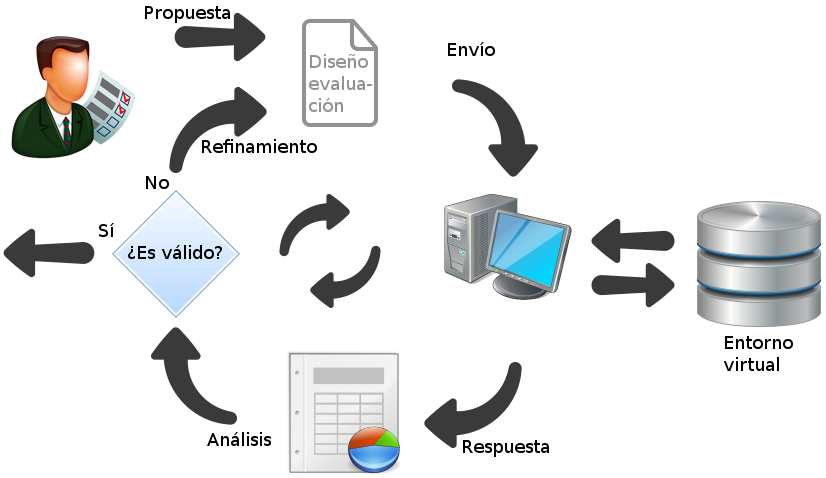
\includegraphics[scale=0.45]{CCHDiagram.png}
  \end{center}
  \caption{Diagrama del ciclo de contraste de hipótesis}
  \label{fig:CCHDiagram}
\end{figure}

\begin{enumerate}
\item \emph{Hipótesis inicial}: el profesor formula una hipótesis para la utilización de algún tipo de información de la actividad de los estudiantes en el entorno virtual para la evaluación de alguna competencia genérica (a). Por ejemplo, se considerará que un estudiante tiene un desempeño correcto de la competencia genérica de planificación y gestión del tiempo si entrega las tareas programadas por el profesor en el VLE con anterioridad a la fecha fijada para las mismas.
\item \emph{Diseño y formulación de evaluación}: el profesor diseñará un indicador para evaluar la competencia a partir de la información del registro y la implementará en la herramienta utilizada para extraer la información (b). Por ejemplo, podríamos considerar partiendo de la hipótesis anterior que un estudiante tendrá un desempeño alto en la competencia de planificación y gestión del tiempo si de las 10 tareas programadas durante el semestre al menos 9 fueron entregadas antes de la fecha fijada para las mismas, un desempeño medio si entregó entre 7 y 8 tareas antes de la fecha fijada y un desempeño bajo si entregó 6 o menos tareas antes de la fecha fijada.
\item \emph{Petición de datos}: Se enviará la petición de datos al sistema encargado de recuperar la información (c). Las herramientas y su funcionamiento serán explicadas más adelante en la sección~\ref{sec:tools}.
\item \emph{Validación de resultados}: la herramienta pondrá a disposición del profesor los indicadores requeridos (d). El profesor los analizará (e) y evaluará si son válidos para el propósito que fueron diseñados (f), si necesitan ser refinados o si hay que descartarlos. En este caso, podrá volver al segundo punto y rediseñar una nueva evaluación (g).
\end{enumerate}

A continuación se presentara un ejemplo para ilustrar el ciclo de contraste de hipótesis. 

\subsubsection*{Ejemplo}

En este ejemplo, el profesor pretende obtener indicadores del uso del foro del entorno virtual para evaluar la competencia genérica de las habilidades interpersonales. Durante el curso, el profesor planteó una actividad de debate mediante el foro de la asignatura que tendría lugar durante una semana de las que conforman el curso. El profesor aplicará dos iteraciones del ciclo de contraste de hipótesis del método DBA.

\paragraph*{Iteración I}

\subparagraph*{I.1 Hipótesis inicial.}

El profesor considera que podría diseñar un indicador válido a partir del número de mensajes que ha escrito cada estudiante en la semana en la que transcurre la actividad y plantea la siguiente hipótesis: \emph{se considerará que un estudiante ha desempeñado satisfactoriamente la competencia genérica de las habilidades interpersonales si ha escrito al menos dos mensajes en el foro}.

\subparagraph*{I.2 Diseño y formulación de la evaluación.}

Para diseñar la evaluación, el profesor deberá contar con un lenguaje cercano al dominio que le permita formular la consulta que le proporcione los indicadores que requiere la hipótesis inicial. En este ejemplo mostramos la consulta~\ref{code:sasqlejemplo1}, escrita en el lenguaje SASQL~\footnote{https://www.assembla.com/spaces/evalcourse/wiki/SASQL} y que proporcionará datos sobre la participación de los estudiantes en el foro entre dos fechas.

\begin{lstlisting}[caption=Participación en el foro en un periodo concreto de tiempo ,label=code:sasqlejemplo1,numbers=left, captionpos=b, morekeywords={Evidence,get, students, show, milestones, participation, access, in, assignment, forum, campus, workshop, interaction, between, and}]
Evidence participacion_foro: 
	get students
	show participation
	in forum between 2015-10-21 and 2015-10-27.
\end{lstlisting}

\subparagraph*{I.3 Petición de datos.}

En este paso, se enviará la consulta a un software que lo interprete, procese y sea capaz de proporcionar al usuario los datos solicitados. %La consulta anterior se introduciría en el software EvalCourse, herramienta creada para este trabajo que acepta consultas escritas en SASQL y se conecta al VLE.

\subparagraph*{I.4 Validación de resultados.}

El software devuelve al profesor los indicadores solicitados mediante el listado~\ref{tab:EvalCourseEj1}. El profesor los analiza y concluye que, en base a la hipótesis inicial, todos los estudiantes menos el 3 (\emph{student3}) habrían desempeñado correctamente la competencia. Sin embargo, el profesor considera pobre esta primera aproximación y decide redefinir la hipótesis inicial.

\begin{table}
	\centering
	\caption{Información sobre la participación en el foro de los estudiantes en un periodo concreto de tiempo}
	\label{tab:EvalCourseEj1}
	\begin{tabular}{|l|l|c|c|c|c|c|}
		\hline
		id & username & Debate-starter & Debate-participation & Total \\
		\hline
		\hline
		1 & student1 & 1 & 2 & 3  \\
		\hline
		2 & student2 & 0 & 4 & 4  \\
		\hline
		3 & student3 & 0 & 1 & 1  \\
		\hline
		4 & student4 & 1 & 2 & 3  \\
		\hline
		5 & student5 & 0 & 2 & 2  \\
		\hline
	\end{tabular}
\end{table}


\paragraph*{Iteración II}

\subparagraph*{II.1 Hipótesis inicial.}

El profesor plantea la nueva hipótesis inicial de la siguiente manera: \emph{se considerará que un estudiante ha desempeñado satisfactoriamente la competencia genérica de las habilidades interpersonales si ha escrito al menos dos mensajes en el foro y ha interactuado con más de un compañero}.

\subparagraph*{II.2 Diseño y formulación de la evaluación.}

El profesor diseña la nueva evaluación mediante la consulta~\ref{code:sasqlejemplo2}.

\begin{lstlisting}[caption=Interacción en el foro en un periodo de tiempo ,label=code:sasqlejemplo2,numbers=left, captionpos=b, morekeywords={Evidence,get, students, show, milestones, participation, access, in, assignment, forum, campus, workshop, interaction, between, and}]
Evidence interacciones_foro: 
	get students
	show interaction
	in forum between 2013-10-21 and 2013-10-27.
\end{lstlisting}

\subparagraph*{II.3 Petición de datos.}

Se introduce la consulta en el software.

\subparagraph*{II.4 Validación de resultados.}

El software devuelve, entre otros formatos, un grafo que muestra las interacciones (figura~\ref{fig:EvalCourseInteraccionForo}). A tenor de los resultados vemos que sólo dos de los estudiantes cumplen la segunda hipótesis (\emph{student2} y \emph{student4}), y bajo esta nueva hipótesis, ellos serian los dos únicos estudiantes que han mostrado un buen desempeño de la competencia genéricas de las habilidades interpersonales.

\begin{figure}
	\centering
	\includegraphics[width=6cm]{{EvalCourseInteraccionForo.png}}
	\caption{Interacción en el foro en un periodo de tiempo.}
	\label{fig:EvalCourseInteraccionForo}
\end{figure}

\section{Características, requisitos y herramienta}

El método DBA para la evaluación de competencias genéricas es un método DBR. Aunque desde el punto de vista del estudiante y considerando la clasificación de métodos de evaluación mostrada en la sección~\ref{sec:methods} diríamos que es un método \emph{evaluación formativo}, ya que permite mejorar el aprendizaje mientras este tiene lugar proporcionando información de manera sistemática y continua. Sin embargo, lo consideramos un método DBR ya que no mejora únicamente la acción del alumno, sino que también es un método de investigación que mejora la acción del profesor.

Mientras que con respecto a la clasificación de técnicas de evaluación mostrada en la sección~\ref{sec:techniques}, la técnica empleada en este método es la de obtención de \emph{indicadores del trabajo en actividades de aprendizaje}.

\subsection{Características}

En el apartado~\ref{sec:dbr} se indican, partiendo del análisis realizado por Terry Andersen y Julie Shattuck~\cite{anderson2012design}, las características que un estudio DBR de calidad debe tener. A continuación se identificará nuestro método DBA en cada una de esas características:

\begin{itemize}
\item \emph{Estar situado en un contexto educativo real}: el método DBA se ha creado en un contexto educativo real (la Universidad de Cádiz) para ser utilizado en este y en otros contextos educativos reales. Su validez será tratada en el capítulo de la evaluación.
\item \emph{Enfocado en el diseño y prueba de una intervención significativa}: La intervención que se lleva a cabo con el método DBA es un \emph{tipo de evaluación}, siendo este uno de los tipos de intervenciones recogidos en la tipología de intervenciones DBR definida por Andersen~\cite{anderson2012design}. 
\item \emph{Empleo de métodos mixtos}: una intervención DBR implica normalmente la aplicación de diferentes métodos, técnicas y herramientas. El método DBA puede combinarse con otros métodos de evaluación con el fin de contrastar evaluaciones y dar validez a los resultados obtenidos con uno u otro método. Por ejemplo, una aplicación de métodos mixtos podría darse en el ejemplo mostrado en el apartado anterior, donde los estudiantes eran evaluados mediante el método DBA de sus habilidades interpersonales. Esa actividad podría formar parte de un conjunto de actividades de trabajo en equipo configuradas por el profesor para realizar una evaluación auténtica. El profesor podría combinar los resultados de la aplicación de ambos métodos y así contrastar los resultados.
\item \emph{Múltiples iteraciones}: el método DBA permite el diseño de evaluaciones y su contraste de resultados (\emph{ciclo de contraste de hipótesis}). A partir de los resultados, el diseño se puede ir refinando iterativamente hasta que los resultados satisfagan las expectativas del profesor o hasta que decida descartarlos por no ser válidos para su evaluación.
\item \emph{Asociación colaborativa entre investigadores y profesores}: el proceso de desarrollo de software es cada vez más colaborativo, tratando de integrar todo lo posible a los usuarios finales para avanzar hacia un proceso dirigido por la comunidad donde tanto los actores técnicos como los no técnicos trabajen juntos para que se cumplan las expectativas. Esto es especialmente apropiado en el campo de los DSLs, herramientas informáticas diseñadas para facilitar el desarrollo de software en un contexto específico~\cite{izquierdo2012community}. Bajo este enfoque se desarrollará el método DBA, colaborando profesores e investigadores en su desarrollo, teniendo así los usuarios finales y expertos en el dominio (los profesores) una participación activa y directa en la definición de una herramienta que implemente el método, es decir, un DSL. 
\item \emph{Evolución de los principios de diseño}: el método DBA permite la creación de diseños para aplicar a diferentes competencias. Ciertos diseños podrían ser definidos como plantillas o patrones para la evaluación de competencias. Estos patrones podrán ser utilizados por otros profesores, y a partir de su reflexión, modificados para ser adaptados a nuevos contextos. De esta forma, los principios y diseños creados por profesores e investigadores no mueren con una práctica, sino que son puntos de partidas para nuevas teorías y experimentos. Por ejemplo, un profesor que trabajase con wikis en sus clases podría utilizar como indicador de un buen desempeño de la competencia de trabajo en equipo el número de contribuciones aportado por cada estudiante a la página de su equipo de trabajo. Un segundo profesor que trabajase con wikis podría mejorar esta evaluación considerando como indicador el peso en bytes de las contribuciones aportadas por cada miembro del equipo. Y un tercer profesor podría mejorar esta evaluación añadiendo un indicador cualitativo de la información aportada al wiki por cada miembro del equipo. Es decir, se parte de un patrón o diseño inicial que los profesores han ido evolucionando para mejorarlo y aplicarlo a su contexto.
\item \emph{Comparación con la investigación-acción}: El objetivo del método DBA, al contrario de lo que ocurre con la investigación-acción, no es sólo alcanzar una serie de objetivos a nivel local, sino que también permite evolucionar a nivel teórico y maximizar la generalización, mejorando así la comprensión de aplicaciones prácticas. Además, permite la participación de un equipo formado por investigadores y profesores mientras que, por lo general, la práctica de la investigación-acción es llevada a cabo únicamente por el profesor que realiza el experimento. Ambos enfoques son muy parecidos y en ocasiones cuesta diferenciarlos. Se podría decir que la investigación-acción carece de ese carácter reflexivo que sí tiene el DBR~\cite{cole2005being}. Para ilustrarlo utilizaremos el ejemplo de la medición de la competencia de trabajo en equipo mediante el wiki mostrado en el punto anterior. En la investigación-acción, un profesor se enfrentaría a esta evaluación por sí solo, sin considerar cómo han evaluado dicha competencia otros en el wiki, sino que adoptaría una solución útil para él en su caso pero que no evolucionaría. Justo al contrario de lo que ocurrió en el ejemplo anterior de wikis, donde cada profesor, investigador o equipo de investigadores y/o profesores tenía en cuenta como había sido abordada antes la evaluación del trabajo en equipo en el wiki y cada nueva evaluación se pudo utilizar como base de futuras evaluaciones.
\item \emph{Repercusión en las prácticas}: El método DBA puede repercutir directamente en las prácticas. A partir de su aplicación en las sesiones prácticas y del análisis de resultados, los investigadores y profesores implicados pueden detectar actividades e interacciones que favorecen el desempeño de competencias y que no habían considerado anteriormente. Esto repercutirá directamente en la organización y programación de actividades en los siguientes cursos.
\end{itemize}

\subsection{Requisitos}

El método debe cumplir una serie de requisitos que parten de los inconvenientes encontrados en la revisión de la literatura realizada en el capítulo \ref{cha:State of the Art} y que han sido resumidos en el capítulo \ref{cha:Problemas}. A continuación se describe cada uno de estos requisitos.

\paragraph*{1. Indicadores objetivos}

Los indicadores reflejan los datos obtenidos directamente del registro de las actividades de aprendizaje, por lo que serán objetivos per se. No ha lugar a consideraciones personales o interpretaciones inexactas de rúbricas cómo ocurría en la autoevaluación o evaluación entre iguales, dónde dos evaluaciones de un mismo trabajo realizadas por personas diferentes podrían tener calificaciones diferentes. En el caso de los indicadores obtenidos del registro de las actividades de aprendizaje, dos estudiantes que tienen los mismos datos en el registro tendrán en el mismo valor en el indicador, y ya será decisión del profesor la interpretación de este indicador en relación con otros indicadores.

\paragraph*{2. Evaluación escalable}

El método para la evaluación de competencias genéricas deberá ser escalable, sin que suponga al profesor un esfuerzo que éste no pueda abordar. El método se alineará con las actividades aprendizaje para que el profesor pueda consultar los indicadores del registro con una simple petición a la herramienta. La herramienta procesará la petición y devolverá la información en formatos que el profesor podrá visionar y exportar a otras herramientas.

\paragraph*{3. Propósito general}

El propósito del método es obtener indicadores del registro de las actividades de aprendizaje y que estos sean utilizados para evaluar competencias genéricas. Pero no están orientados a una competencia genérica concreta, sino que es el profesor quien diseña sus actividades en el entorno virtual y el que luego obtiene los indicadores para después utilizarlos en la evaluación de la competencia genérica que considera que los estudiantes han desempeñado en dicha tarea (y que queda reflejada en los indicadores). El profesor podría incluso utilizar los indicadores para evaluar competencias específicas si lo creyese oportuno. Pero en ningún caso este método tiene como propósito una competencia y actividad concreta como ocurría, por ejemplo, con algunos juegos serios recogidos en el estado del arte.

\paragraph*{4. Accesibilidad}

No deberá ser un requisito que el profesor tenga un perfil informático u otro específico para poder realizar las peticiones de los indicadores, ni que contrate a un equipo de expertos para obtener los indicadores. La interfaz en la que se implementará el método debe ser usable y sencilla para que los profesores puedan utilizarla sin requerirles conocimientos técnicos, y los formatos a los que se exporte la información serán figuras y documentos en formatos transportables a cualquier hoja de cálculo.

\paragraph*{5. Diseño de evaluaciones}

La herramienta proporciona al profesor la posibilidad de diseñar sus propias evaluaciones a partir de los indicadores. En el estado del arte nos encontramos con trabajos que obtenían sus evaluaciones a partir de los indicadores del VLE, pero éstos eran fijos. Es decir, cada competencia se evaluaba con un indicador dado. Pero podía ocurrir que el profesor no utilizase las actividades del VLE que proporcionaban dichos indicadores o que plantease las actividades con un enfoque diferente al que realmente tienen. Por ejemplo, uno de los puntos fuertes de un wiki es que favorecen el trabajo colaborativo, y podríamos encontrar herramientas que nos ayuden a valorar el trabajo en equipo de los estudiantes que participan en una página de un wiki mediante indicadores del trabajo colaborativo. Si un profesor plantea actividades en el wiki de manera que cada estudiante trabaje individualmente en una página, podrá valorar otras competencias, pero el trabajo en equipo no. Con este método el profesor es quién diseña sus indicadores, y por tanto, sus evaluaciones a partir de los registros de las actividades de aprendizaje.

En resumen, podemos decir que el método que se propone para evaluar competencias genéricas a partir de los registros de interacción de las actividades de aprendizaje se pone a disposición del profesor en forma de una herramienta informática que se conecta a la actividad de aprendizaje utilizado en la asignatura. Mediante esta herramienta, los profesores pueden diseñar evaluaciones a partir de indicadores objetivos obtenidos del VLE y aplicarlos a las competencias genéricas para las que ellos consideren que les son válidos.

\subsection{Herramienta}

La herramienta que implemente el método debe cumplir una serie de requisitos que ayuden a alcanzar los mencionados en el punto anterior:

\begin{itemize}
\item \emph{Cercana al dominio}: la herramienta debe servir al profesor o investigador para definir indicadores a partir de la actividad de los estudiantes en los entornos de aprendizaje, por tanto, debe ser una herramienta definida en términos del ámbito educativo.
\item \emph{Personalización de evaluaciones}: la herramienta debe proporcionar un mecanismo para permitir al usuario crear sus diseños a partir de los indicadores disponibles en el entorno virtual.
\item \emph{Usabilidad}: la herramienta debe ser usable por usuarios de perfil no informático, por lo que su utilización debe ser sencilla y entendible por este tipo de usuarios.
\end{itemize}

A tenor de estos requisitos se decidió que la herramienta informática a implementar sería un \emph{lenguaje específico de dominio} (\emph{DSL}, del inglés, \emph{domain-specific language}). Un DSL es un lenguaje de programación orientado a un dominio concreto. Estos se han vuelto muy populares en los últimos años, y una de las principales razones es que facilitan la comunicación con los expertos en el dominio, proporcionando un texto común (código escrito en el DSL) que actúa a la vez como ejecutable y como una descripción que los expertos en el dominio pueden leer para entender como sus ideas se representan en el sistema~\cite{fowler2010domain}. En el método DBA, el ejecutable sería el diseño y los expertos en el dominio los profesores.



% La evaluación de las 3 herramientas se corresponde al capítulo siguiente.


%Metodología mixta

%Cómo voy a evaluar roles, momentos, actividad, ... lo que sea.

%Explicar el DSL

%DSL: herramienta de investigación en evaluaciones. Esta herramienta ayuda al investigador a formalizar la evaluación.
 
%Enfocar la metodología a que no es una metodología para evaluar, sino para diseñar evaluaciones. Diseñador de evaluaciones.

%Explicar qué pasos tiene que seguir un diseñador de evaluaciones para hacer sus evaluaciones.

%Dentro de los resultados obtenemos dos cosas:
%1. Diseño
%2. Lo que el diseñador nos indicó que no pudo hacer

%Para que esto sea posible falta la herramienta informática

%\section{Evolución herramientas}

%AMW --> EvalCourse --> EvalSim

%\section{Metodología de desarrollo}

%DSL? Ing. Dirigida x modelo?



%------------------------------------------------------------------------------------------------------------------------------------------------

